\documentclass{article}
\usepackage{style-assessments}

% define macros (/shortcuts)
\newcommand{\bu}[1]{\textbf{\ul{#1}}}				% shortcut bold and underline text in one command
\newcommand{\ind}{\perp \!\!\! \perp}			% define independence symbol (it basically makes two orthogonal symbols very close to each other. The number of \! controls the space between each of the orthogonal symbols)
\newcommand{\integral}[4]{\displaystyle \int_{#1}^{#2} #3 \,\mathrm{d} #4}		% shortcut for large integral with limits and appending formatted dx (variable x)
\newcommand{\e}{\mathrm{e}}		% shortcut for non-italic e in math mode
\newcommand{\gam}[1]{\Gamma(#1)}		% shortcut for gamma function (variable)
\newcommand{\Beta}[2]{B(#1, #2)}		% shortcut for beta function B(variable1, variable 2)
\newcommand{\follow}[1]{\sim \text{#1}\,}		% shortcut for ~ 'Named dist ' in normal font with space before parameters would go
\newcommand{\followsp}[2]{\overset{#1}\sim \text{#2}\,}		% (followsp is short for 'follow special') shortcut that can be used for iid or ind ~ 'Named dist ' in normal font with space before parameters would go
\newcommand{\cov}[1]{\mathrm{Cov}(#1)}		% shortcut for Cov(X,Y) with formatting for Cov
\newcommand{\corr}[1]{\mathrm{Corr}(#1)}		% shortcut for Corr(X,Y) with formatting for Corr
\newcommand{\vecn}[2]{#1_1, \ldots, #1_{#2}}	% define vector (without parentheses, so when writing out in like a definition) of the form X_1, ..., X_n, where X and n are variable. NOTE: to call use $\vecn{X}{k}$
\newcommand{\chisq}{\raisebox{2pt}{$\chi^2$}}		% shortcut for chi-square distribution (better formatted chi letter in math mode with square added)
\newcommand{\order}[2]{#1_{(#2)}}		% shortcut for order stat notation X_{(j)} (random variable and subscript variable)
\newcommand{\convp}[2]{#1 \overset{p} \to #2}		% shortcut for Xn converges to X in probability (with arrow notation)
\newcommand{\ho}{H_0}		% shortcut for null hypothesis formatted nicely
\newcommand{\ha}{H_A}		% shortcut for alternative hypothesis formatted nicely



\begin{document}

\begin{center}
{\Huge MATH 321: Final Study Guide}

\end{center}

\bigskip\bigskip

{\large \bu{Lecture 14 -- Bivariate Distributions}} (4.1 and 4.4)\bigskip

Joint pmf and pdf
\begin{itemize}
    \item Discrete definition: The joint pmf is defined as $f(x,y) = P(X = x, Y = y)$ for all $(x, y) \in \mathbb{R}^2$ and has properties
    \begin{enumerate}
        \item $0 \le f_{X,Y}(x,y) \le 1$ \quad for all $x, y$
        \item $\displaystyle \sum_x \sum_y f(x,y) = \sum_y \sum_x f(x,y) = 1$
        \item Let $A$ be any subset of $\mathbb{R}^2$, then $\displaystyle P((X,Y) \in A) = {\sum \sum}_A f(x,y)$
    \end{enumerate}
    \item Continuous definition: The joint pdf is a function $f(x,y)$ from $\mathbb{R}^2$ into $\mathbb{R}$ such that
    \begin{enumerate}
        \item $f_{X,Y}(x,y) \ge 0$ \quad for all $x, y$
        \item $\integral{-\infty}{\infty}{\integral{-\infty}{\infty}{f(x,y)}{x}}{y} = \integral{-\infty}{\infty}{\integral{-\infty}{\infty}{f(x,y)}{y}}{x} = 1$
        \item For $A \subset \mathbb{R}^2$, $\displaystyle P((X,Y) \in A) = \integral{}{}{\integral{A}{}{f(x,y)}{x}}{y} = \integral{}{}{\integral{A}{}{f(x,y)}{y}}{x}$
    \end{enumerate}
\end{itemize}\bigskip

Marginal distributions
\begin{itemize}
    \item Discrete definition: Let $(X,Y)$ have joint pmf $f(x,y)$. Then, the marginal pmfs are given by
    \item[] $\displaystyle f_X(x) = \sum_y f_{X,Y}(x,y) \hspace{20pt} \text{and} \hspace{20pt} f_Y(y) = \sum_x f_{X,Y}(x,y)$
    \item Continuous definition: Let $(X,Y)$ have joint pdf $f(x,y)$. Then the marginal pdfs are defined by:
    \item[] $f_X(x) = \integral{-\infty}{\infty}{f(x,y)}{y} \hspace{20pt} \text{and} \hspace{20pt} f_Y(y) = \integral{-\infty}{\infty}{f(x,y)}{x}$
\end{itemize}\bigskip

Expected values of a function of a random variable
\begin{itemize}
    \item Definition: Let $g(X,Y)$ be a function of a bivariate random vector $(X,Y)$.
    \begin{enumerate}[(a)]
        \item If $X$ and $Y$ are discrete with joint pmf $f(x,y)$,
        \item[] $\displaystyle E[g(X,Y)] = \sum_x \sum_y g(x,y) f(x,y)$
        \item If $X$ and $Y$ are continuous with joint pdf $f(x,y)$,
        \item[] $\displaystyle E[g(X,Y)] = \integral{-\infty}{\infty}{\integral{-\infty}{\infty}{g(x,y) f(x,y)}{x}}{y}$
    \end{enumerate}
\end{itemize}\bigskip

\newpage

Special expectations
\begin{itemize}
    \item Definitions: Let $(X_1,X_2)$ be a bivariate random vector with joint pmf / pdf $f(x_1,x_2)$.
    \begin{enumerate}[i)]
        \item If $g(X_1,X_2) = X_1$, then $E[g(X_1,X_2)] = E(X_1) = \mu_{X_1}$ 
        \item If $g(X_1,X_2) = (X_1 - \mu_1)^2$, then $E[g(X_1,X_2)] = E[(X_1 - \mu_1)^2]  = \sigma_{X_1}^2$ 
        \item If $g(X_1,X_2) = \e^{tX_1}$, then $E[g(X_1,X_2)] = E(\e^{tX_1}) = M_{X_1}(t)$
    \end{enumerate}
\end{itemize}\bigskip

Expected value of $X + Y$ and $XY$
\begin{itemize}
    \item Theorem: Expected value of a sum of two random variables
    \item[] If $g(X,Y) = X + Y$, then $E(X + Y) = E(X) + E(Y)$
    \item Generalized theorem: If $g_1(X,Y)$ and $g_2(X,Y)$ are two functions and $a$, $b$ and $c$ are constants, then
    \item[] $E[ag_1(X,Y) + bg_2(X,Y) + c] = aE[g_1(X,Y)] + bE[g_2(X,Y)] + c$
    \item Theorem: Expected value of a product of two random variables
    \item[] If $g(X,Y) = XY$ and $X \ind Y$, then $E(XY) = E(X) \cdot E(Y)$
\end{itemize}\bigskip\bigskip

{\large \bu{Lecture 15 -- Conditional Distributions}} (4.3)\bigskip

Conditional pmf / pdf
\begin{itemize}
    \item Definition: Let $(X,Y)$ be a bivariate random vector with joint pmf / pdf $f(x,y)$ and marginal pmfs / pdfs $f_X(x)$ and $f_Y(y)$.
    \begin{enumerate}[(a)]
        \item Given $x$ such that $f_X(x) > 0$, \hspace{20pt} $\displaystyle f(y \mid x) = \frac{f(x,y)}{f_X(x)}$
        \item Given $y$ such that $f_Y(y) > 0$, \hspace{20pt}  $\displaystyle f(x \mid y) = \frac{f(x,y)}{f_Y(y)}$
    \end{enumerate}
\end{itemize}\bigskip

Probabilities
\begin{itemize}
    \item For $A \subset \mathbb{R}^2$,
    \item[] Discrete: $\displaystyle P(X \in A \mid Y = y) = \sum_{x \in A} P(X = x \mid Y = y) = \sum_{x \in A} f(x \mid y)$
    \item[] Continuous: $P(X \in A \mid Y = y) = \integral{A}{}{f(x \mid y)}{x}$
\end{itemize}\bigskip

Relationship between joint pmf and conditional pmfs
\begin{itemize}
    \item Theorem: For bivariate random vector $(X,Y)$ with joint pmf / pdf $f(x,y)$ and $x$ and $y$ such that $f_X(x) > 0$ and $f_Y(y) > 0$,
    \item[] $f(x, y) = f_Y(y) \cdot f(x \mid y) =  f_X(x) \cdot f(y \mid x)$
\end{itemize}\bigskip

\newpage

Conditional expected values
\begin{itemize}
    \item Definition: Let $g(Y)$ be a function of $Y$, then the conditional expected value of $g(Y)$ given that $X = x$ is given by 
    \item[] $\displaystyle E[g(Y) \mid x ] = \sum_y g(y) f(y \mid x) \hspace{20pt} \text{and} \hspace{20pt} E[g(Y) \mid x] = \integral{-\infty}{\infty}{g(y) f(y \mid x)}{y}$
    \item Conditional mean and variance definitions (assuming $X$ and $Y$ are discrete):
    \begin{enumerate}[i)]
        \item If $g(Y) = Y$, then the conditional mean of $Y$ given $X = x$ is
        \item[] $\displaystyle E(Y \mid X = x) = \sum_y y \, f(y \mid x) = \mu_{Y \mid X}$
        \item If $g(Y) = (Y - \mu_{Y\mid X})^2$, then the conditional variance of $Y$ given $X = x$ is
        \item[] $\displaystyle E[(Y - \mu_{Y \mid X})^2 \mid X = x] = \sum_y (y - \mu_{Y \mid X})^2 \, f(y \mid x) = \sigma_{Y \mid X}^2$
    \end{enumerate}
\end{itemize}\bigskip

\vspace{100pt}

{\large \bu{Lecture 16 -- Independence and the Correlation Coefficient}} (4.1, 4.2, and 4.4)\bigskip

Independence for random variables\bigskip
\begin{itemize}
    \item Definition: Let $(X,Y)$ be a bivariate random vector with joint pdf / pmf $f(x,y)$ and marginal pdfs / pmfs $f_X(x)$ and $f_Y(y)$. Then $X$ and $Y$ are called independent random variables if, for every $x \in \mathbb{R}$ and $y \in \mathbb{R}$,
    \item[] $f(x,y) = f_X(x) \cdot f_Y(y)$
    \item Checking independence theorem: $X$ and $Y$ are independent random variables if and only if 
    \item[] $f(x,y) = g(x) \cdot h(y), \quad\quad a \le x \le b, \, c \le y \le d$,
    \item[] where $g(x)$ is a nonnegative function of $x$ alone and $h(y)$ is a nonnegative function of $y$ alone
\end{itemize}\bigskip

Conditional distributions and independence
\begin{itemize}
    \item Theorem: If $X$ and $Y$ are independent, $f(x \mid y) = f_X(x) \hspace{25pt} \text{and} \hspace{25pt} f(y \mid x) = f_Y(y)$
\end{itemize}\bigskip

Using independence
\begin{itemize}
    \item Theorem: Let $X$ and $Y$ be independent random variables.
    \begin{enumerate}[(a)]
         \item For any $A \subset \mathbb{R}$ and $B\subset \mathbb{R}$, $P(X \in A,Y \in B) = P(X \in A) \cdot P(Y \in B)$
        \item Let $g(x)$ be a function only of $x$ and $h(y)$ be a function only of $y$. Then
        \item[] $E[g(X) \cdot h(Y)] = E[g(X)] \cdot E[h(Y)]$
    \end{enumerate}
\end{itemize}\bigskip\bigskip

Definition, theorems and properties of covariance
\begin{itemize}
    \item Definition: The covariance of $X$ and $Y$ is the number defined by: $\cov{X,Y} = E[(X - \mu_X)(Y - \mu_Y)]$
        \item If $(X,Y)$ is discrete, then $E[(X - \mu_X)(Y - \mu_Y)] = \sum_x \sum_y (x - \mu_x)(y - \mu_y \, f(x,y)$
        \item Alternate calculation for covariance: $\cov{X,Y} = E(XY) - E(X) \cdot E(Y)$
        \item Variance is a special case of covariance: $V(X) = \cov{X,X}$
        \item Order in covariance does not matter (i.e. symmetric): $\cov{X,Y} = \cov{Y,X}$
        \item Covariance of a random variable and a constant is zero: If $c$ is a constant, then $\cov{X,c} = 0$
        \item Can factor out coefficients in covariance: $\cov{aX,bY} = ab \cdot \cov{X,Y}$
        \item Can factor out coefficients, but added constants disappear: $\cov{aX + c,bY + d} = ab \cdot \cov{X,Y}$
        \item Distributive property of covariance: $\cov{X, Y + Z} = \cov{X,Y} + \cov{X,Z}$
        \item Independence and covariance theorem: If $X \ind Y$ then $\cov{X,Y} = 0$
\end{itemize}\bigskip

Correlation definition and properties
\begin{itemize}
    \item Definition: $\displaystyle \rho_{XY} = \corr{X,Y} = \frac{\cov{X,Y}}{\sqrt{V(X) V(Y)}} = \frac{\cov{X,Y}}{\sigma_X \sigma_Y}$
    \item Theorem: For any random variable $X$ and $Y$,
    \begin{enumerate}[i)]
        \item $-1 \le \rho_{XY} \le 1$ 
        \item $\rho_{XY} = 1$ if and only if there exist numbers $a > 0$ and $b$ such that $P(Y = aX + b) = 1$.
        \item $\rho_{XY} = -1$ if and only if there exist numbers $a < 0$ and $b$ such that $P(Y = aX + b) = 1$. 
        \item When $\rho_{XY} = 0$, $X$ and $Y$ are uncorrelated.
    \end{enumerate}
\end{itemize}\bigskip

Variance of $X + Y$
\begin{itemize}
    \item Theorem: Variance of a sum of two random variables
    \item[] $V(X + Y) = V(X) + V(Y) + 2 \,\cov{X,Y}$
    \item[] If $X \ind Y$, then $V(X + Y) = V(X) + V(Y)$
\end{itemize}\bigskip

\newpage

{\large \bu{Lecture 17 -- Several Random Variables}} (5.3 and 5.4)\bigskip

Definitions and theorems
\begin{itemize}
    \item Joint distributions
    \begin{itemize}
        \item Discrete definition: If $\mathbf{X} = (\vecn{X}{n})$ a discrete random vector (the range is countable), then the joint pmf of $\mathbf{X}$ is the function defined by
        \item[] $f(\mathbf{x}) = f(\vecn{x}{n}) = P(X_1 = x_1, \ldots, X_n = x_n) \text{ for each } (\vecn{x}{n}) \in \mathbb{R}^n$
        \item[] Then for any $A \subset \mathbb{R}^n$,
        \item[] $\displaystyle P(\mathbf{X} \in A) = \sum_{\mathbf{x} \in A} f(\mathbf{x})$
        \item Continuous definition: If $\mathbf{X} = (\vecn{X}{n})$ a continuous random vector, then the joint pdf of $\mathbf{X}$ is the function $f(\mathbf{x}) = f(\vecn{x}{n})$ that satisfies
        \item[] $P(\mathbf{X} \in A) = \int \cdots \integral{A}{}{f(\mathbf{x})}{\mathbf{x}} = \int \cdots \int_A f(\vecn{x}{n}) \mathrm{d}x_1\cdots \mathrm{d}x_n$
    \end{itemize}
    \item Expected values: Let $g(\mathbf{x})$ be a real-valued function defined on the range of $\mathbf{X}$. The expected value of $g(\mathbf{X})$ is\\
    \begin{tabular}{c c c c}
        & \ul{Discrete} & \ul{Continuous}\\
        $E[g(\mathbf{X})] = $ & $\displaystyle \sum_{\mathbf{x} \in \mathbb{R}^n} g(\mathbf{x}) f(\mathbf{x})$ & $\displaystyle \int_{-\infty}^{\infty} \cdots \int_{-\infty}^{\infty} g(\mathbf{x}) f(\mathbf{x}) \mathrm{d}x_1\cdots \mathrm{d}x_n$\\
    \end{tabular}\bigskip
    \item Marginal distributions: The marginal pdf or pmf of any subset of the coordinates of $(\vecn{X}{n})$ can be computed by integrating or summing the joint pdf or pmf over all possible values of the other coordinates.
    \item Conditional distributions: The conditional pmf or pdf of a subset of the coordinates of $(\vecn{X}{n})$ given the value of the remaining coordinates is obtained by dividing the joint pdf or pmf by the marginal pdf or pmf of the remaining coordinates.
\end{itemize}\bigskip

Independence
\begin{itemize}
    \item Definition: Let random variables $\vecn{X}{n}$ have joint pdf (or pmf) $f(\vecn{x}{n})$ and let $f_{X_i}(x_i)$ be the marginal pdf (or pmf) of $X_i$. Then $\vecn{X}{n}$ are mutually independent random variables if, for every $(\vecn{x}{n})$, the joint pdf (or pmf) can be written as
    \item[] $\displaystyle f(\vecn{X}{n}) = f_{X_1}(x_1) \cdots f_{X_n}(x_n) = \prod_{i = 1}^n f_{X_i}(x_i)$
    \item Conditional distributions: If $\vecn{X}{n}$ are mutually independent, the conditional distribution of any subset of the coordinates, given the values of the rest of the coordinates, is the same as the marginal distribution of the subset.
    \item Expected value: Let $\vecn{X}{n}$  be mutually independent random variables. Let $\vecn{g}{n}$ be real-valued functions such that $g_i(x)$ is a function only of $x_i$, $i = 1, \dots, n$. Then
    \item[] $\displaystyle E[g_1(X_1) \cdots g_n(X_n)] = \prod_{i = 1}^n E[g_i(x_i)]$
\end{itemize}\bigskip

\newpage

Linear functions of random variables
\begin{itemize}
    \item Definition: A linear function of random variables consists of $n$ random variables $\vecn{X}{n}$ and $n$ coefficient $\vecn{a}{n}$
    \item[] $\displaystyle a_1 X_1 + a_2 X_2 + \cdots + a_n X_n = \sum_{i = 1}^n a_i X_i$
    \item Expected value of a linear function of random variables
    \item[] $E[a_1 X_1 + a_2 X_2+ \cdots + a_n X_n] = a_1 E(X_1) + a_2 E(X_2) + \cdots + a_n E(X_n)$
    \item Variance of a linear function of random variables
    \item[] $\displaystyle V[a_1 X_1 + a_2 X_2+ \cdots + a_n X_n] = \sum_{i = 1}^n a_i^2 V(X_i) + 2 \sum_{i < j} a_i a_j \cov{X_i,X_j}$
    \item[] If $\vecn{X}{n}$ are mutually independent,
    \item[] $\displaystyle V[a_1 X_1 + a_2 X_2+ \cdots + a_n X_n] = \sum_{i = 1}^n a_i^2 V(X_i)$
\end{itemize}\bigskip

Mgf of sums of independent random variables
\begin{itemize}
    \item Theorem: Let $\vecn{X}{n}$ be mutually independent random variables with mgfs $M_{X_1}(t), \ldots, M_{X_n}(t)$. Let $Y = X_1 + \cdots + X_n$.
    \item[] $\displaystyle M_Y(t) = M_{X_1 + \cdots + X_n}(t) = M_{X_1}(t) \cdots M_{X_n}(t) = \prod_{i = 1}^n M_{X_i}(t)$
    \item[] If $\vecn{X}{n}$ all have the same distribution with mgf $M_X(t)$, then
    \item[] $M_Y(t) = \big[M_X(t)\big]^n$
\end{itemize}\bigskip

Sums of linear combinations of random variables
\begin{itemize}
     \item Theorem: Let $\vecn{X}{n}$ be mutually independent random variables with mgfs $M_{X_1}(t), \ldots, M_{X_n}(t)$. Let $\vecn{a}{n}$ and $\vecn{b}{n}$ be fixed constants. Let $Y = (a_1 X_1 + b_1) + \cdots + (a_n X_n + b_n)$. Then the mgf of $Y$ is
     \item[] $M_Y(t) = \big(\e^{t \sum b_i}\big) M_{X_1}(a_1 t) \cdots M_{X_n}(a_n t)$
     \item Sum of linear function of normals theorem: Let $\vecn{X}{n}$ be mutually independent random variables with $X_i \follow{Normal}(\mu_i, \sigma_i^2)$. Let $\vecn{a}{n}$ and $\vecn{b}{n}$ be fixed constants. Then,
     \item[] $\displaystyle Y =\sum_{i = 1}^n (a_i X_i + b_i) \follow{Normal}\bigg(\mu = \sum_{i = 1}^n (a_i \mu_i + b_i), \, \sigma^2 = \sum_{i = 1}^n a_i^2 \sigma_i^2\bigg)$
\end{itemize}\newpage

{\large \bu{Lecture 1 -- Random Samples and Common Statistics}} (5.5)\bigskip

Basic concepts of random samples
\begin{itemize}
    \item Random sample definition: $\vecn{X}{n}$ are a random sample of size $n$ from the population $f(x)$ if they are $iid$ random variables.
    \item Statistic (estimator) definition: The random variable / vector for any function of a random sample $Y = T(\vecn{X}{n})$ is called a statistic, and it's distribution is called a sampling distribution.
\end{itemize}\bigskip

Sample mean and variance
\begin{itemize}
    \item Definitions
    \begin{itemize}
        \item Sample mean: The arithmetic average of the values in a random sample
        \item[] $\displaystyle \bar{X} = \frac{X_1 + \cdots + X_n}{n} = \frac{1}{n} \sum_{i = 1}^n X_i$
        \item Sample variance: The statistic defined by $\displaystyle S^2 = \frac{1}{n - 1} \sum_{i = 1}^n (X_i - \bar{X})^2$
        \item Sample standard deviation: The statistic defined by $S = \sqrt{S^2}$
    \end{itemize}
    \item Theorem: Let $\vecn{X}{n}$ be a random sample of size $n$ from a population with mean $\mu$ and variance $\sigma^2 < \infty$. Then
    \item[] (a) $\mu_{\bar{X}} = E(\bar{X}) = \mu$ \hspace{20pt} (b) $\sigma_{\bar{X}}^2 = V(\bar{X}) = \frac{\sigma^2}{n}$ \hspace{20pt} (c) $E(S^2) = \sigma^2$
    \item Sampling distribution of $\bar{X}$ from random sample $\vecn{X}{n}$
    \item[] Theorem: Mgf of the sample mean is $M_{\bar{X}}(t) = [M_X(t / n)]^n$
\end{itemize}\bigskip
     
Sampling from the normal distribution
\begin{itemize}
    \item Let $\vecn{X}{n}$ be a random sample of size $n$ from a $\text{Normal }(\mu, \sigma^2)$ distribution. Then
    \item[] (a) $\bar{X} \ind S^2$ \hspace{20pt} (b) $\bar{X} \follow{Normal}(\mu, \frac{\sigma^2}{n})$ \hspace{20pt} (c) $\displaystyle \frac{(n-1)}{\sigma^2} S^2  \follow{\chisq}(n-1)$
\end{itemize}\bigskip

Chi-square random variables
\begin{itemize}
    \item If $Z \follow{Normal}(0, 1)$, then $Z^2 \follow{\chisq}(1)$ $\rightarrow$ $\displaystyle \big(\frac{\bar{X} - \mu}{\sigma}\big)^2 = Z^2 \follow{\chisq}(1)$
    \item Additive $df$: If $\vecn{X}{n}$ are mutually independent and $X_i \follow{\chisq}(r_i)$ for $i = 1, \ldots, n$, then \\ $Y = X_1 + \cdots + X_n \follow{\chisq}(r_1 + \cdots + r_n)$
    \item Result / extension of this: If $\vecn{X}{n}$ are mutually independent random variables with \\ $X_i \follow{Normal}(\mu_i, \sigma_i)$ for $i = 1, \ldots, n$, then
    \item[] $\displaystyle \sum_{i=1}^n \big(\frac{\bar{X} - \mu}{\sigma}\big)^2 = \sum_{i=1}^n Z^2 \follow{\chisq}(n)$
\end{itemize}\bigskip

\newpage

$t$ distribution
\begin{itemize}
    \item Definition: Let $\vecn{X}{n}$ be a random sample from a $N(\mu, \sigma^2)$ population. Then $\displaystyle \frac{\bar{X} - \mu}{S / \sqrt{n}} \follow{$t$}_{n-1}$
    \item Derivation: $\displaystyle \frac{Z}{\sqrt{\chisq_r / r}} \follow{$t$}_r$
\end{itemize}\bigskip

$F$ distribution
\begin{itemize}
    \item Definition: Let $\vecn{X}{n}$ be a random sample from a $N(\mu_X, \sigma^2_X)$ population, and let $\vecn{Y}{m}$ be a random sample from an independent $N(\mu_Y, \sigma^2_Y)$ population. If
    \item[] $\displaystyle W = \frac{S^2_X / S^2_Y}{\sigma^2_X / \sigma^2_Y} \hspace{20pt} \text{then} \hspace{20pt} W \follow{$F$}(n-1, m-1)$. In general, $W \follow{$F$}(r_1, r_2)$.
    \item Derivation: $\displaystyle \frac{\chisq_{r_1} / r_1}{\chisq_{r_2} / r_2} \follow{$F$}(r_1, r_2)$
    \item Relationship to other distributions theorem
    \item[] (a) If $X \follow{$F$}(r_1,r_2)$ then $1/X \follow{$F$}(r_2,r_1)$ \hspace{20pt} (b) If $X \follow{$t$}_r$ then $X^2 \follow{$F$}(1,r)$
\end{itemize}\bigskip

\vspace{50pt}

{\large \bu{Lecture 2 -- Order Statistics}} (6.3)\bigskip

Order statistics definition and distributions
\begin{itemize}
    \item Definition: The order statistics are random variables that satisfy $\order{X}{1} \le \cdots \le X_{(n)}$. In particular
    \begin{align*}
    \order{X}{1} &= \min_{1 \le i \le n} X_i,\\
    \order{X}{2} &= \text{second smallest } X_i\\
    &\vdots\\
    \order{X}{n} &= \max_{1 \le i \le n} X_i.
    \end{align*}
    \item Distribution theorems
    \begin{itemize}
        \item Cdf: 
        \begin{align*}
        F_{\order{X}{j}}(x) &= P(\order{X}{j} \le x) = \sum_{k = j}^n {n \choose k} [F_{X}(x)]^k [1- F_X(x)]^{n - k}\\
        &= P(Y \le j), \quad \text{where} \quad Y \follow{Binomial}(n, p = P(X \le x) = F_X(x))
        \end{align*}
        \item Pdf:
        \begin{align*}
        f_{\order{X}{j}}(x) &= \frac{n!}{(j - 1)!(n - j)!} \, [F_X(x)]^{j - 1} \, f_X(x) \, [1 - F_X(x)]^{n - j}\\
        &= [\text{multinomial coefficient}] \times [j-1 \text{ RVs } \le x] \times [1 \text{ RV} \approx x] \times [n-j \text{ RVs } > x] 
        \end{align*}
    \end{itemize}
    \item $f_{\order{X}{j}}(x) = F'_{\order{X}{j}}(x)$
    \item Extreme order stats\medskip\\
    \begin{tabular}{l l l l }
    Min \hspace{10pt} & $\rightarrow$ \hspace{10pt} & $F_{\order{X}{1}}(x) = 1 - [1 - F_X(x)]^n$; & $f_{\order{X}{1}}(x) = n f_X(x) [1 - F_X(x)]^{n-1}$\\\\
    Max \hspace{10pt} & $\rightarrow$ \hspace{10pt} & $F_{\order{X}{n}}(x) = [F_X(x)]^n$; & $f_{\order{X}{n}}(x) = n [F_X(x)]^{n-1} f_X(x)$
    \end{tabular}
\end{itemize}\bigskip

Specific order statistics and functions of order statistics
\begin{itemize}
    \item Sample median $M$
    \[M =
    \left\{
    \begin{array}{ll}
        \order{X}{\frac{n+1}{2}} & \text{if $n$ is odd}\\
        \big[\order{X}{\frac{n}{2}} + \order{X}{\frac{n}{2} + 1}\big] / 2 & \text{if $n$ is even}\\
    \end{array}
    \right.\]
    \item Sample range, $R = \order{X}{n} - \order{X}{1} = max(\vecn{X}{n}) - min(\vecn{X}{n})$
    \item $IQR = Q_3 - Q_1$
    \item $\displaystyle \text{Midrange} = \frac{\order{X}{1} + \order{X}{n}}{2}$
\end{itemize}\bigskip

Order statistics as estimators of population percentiles
\begin{itemize}
    \item Expected value of the ``position'' of order statistics theorem
    \item[] If $\order{X}{1}, \ldots, \order{X}{n}$ are order statistics, then $\displaystyle E[F_X(\order{X}{j})] = \frac{j}{n+1}, \quad j = 1, \ldots, n$
    \item[] Can use $\order{X}{j}$ as an estimator of $x_p$, where $p = j / (n+1)$.
\end{itemize}\bigskip

q--q plots
\begin{itemize}
    \item Expected probability between two adjacent order statistics theorem:
    \item[] $E[F_X(\order{X}{j}) - F_X(\order{X}{j-1})] = \frac{1}{n+1}$; \hspace{20pt}$E[F_X(\order{X}{1})] = \frac{1}{n+1}$; \hspace{20pt} $E[1 - F_X(\order{X}{n})] = \frac{1}{n+1}$
    \item q--q plot definition: Let $\order{x}{1}, \dots, \order{x}{n}$ be the observed sample order statistics and $x_{\frac{1}{n+1}}, \ldots, x_{\frac{n}{n+1}}$ be the percentiles from some particular distribution. A q--q plot is a plot of the points
    \item[] $(\order{x}{1}, x_{\frac{1}{n+1}}) \,\, , \,\, \ldots \,\, , \,\, (\order{x}{n}, x_{\frac{n}{n+1}})$
    \item Interpretation of a q--q plot
    \item[] Good model $\rightarrow$ Follows $y = x$ line.
    \item[] Bad model $\rightarrow$ Strong deviation from this line.
    \item q--q plots for the normal distribution.
    \item[] If plot $(\order{x}{1}, z_{\frac{1}{n+1}}) \,\, , \,\, \ldots \,\, , \,\, (\order{x}{n}, z_{\frac{n}{n+1}})$, then $\frac{1}{\text{slope}} \approx \sigma$
\end{itemize}\bigskip

\newpage

{\large \bu{Lecture 3 -- Exploratory Data Analysis}} (6.2)\bigskip

Univariate EDA
\begin{itemize}
    \item Descriptive statistics: Goal is to summarize a whole dataset wtih a single or few measures
    \begin{itemize}
        \item Sample mean $\displaystyle \bar{x} = \frac{1}{n} \sum_{i = 1}^n x_i$
        \item Sample variance: $\displaystyle s^2 = \frac{1}{n - 1} \sum_{i = 1}^n (x_i - \bar{x})^2 = \frac{n}{n - 1} v$
        \item Data (or population) variance: $\displaystyle v = \frac{1}{n} \sum_{i = 1}^n (x_i - \bar{x})^2$
    \end{itemize}
    \item Displaying data
    \begin{itemize}
        \item Frequency tables: Data is grouped into intervals of equal length (bins)
        \item[] Freq = count of observations in each; Relative freq = proportion of observations in each bin = Freq / $n$
        \item Histograms: Shape and summary stats\smallskip\\
        \begin{tabular}{rlllll}
            Right-skewed: & mean & > & median & > & mode \\
            Symmetric: & mean & $\approx$ & median & $\approx$ & mode \\
            Left-skewed: & mean & < & median & < & mode \\
        \end{tabular}
        \item Density histograms: Estimate underlying pdf
        \item[] For constants $c_1$ and $c_2$, $P(c_1 \le X < c_2) \approx  \frac{\text{Freq}}{n}$ on $(c_1, c_2]$
        \item[] Height of bar $h(x) = \frac{\text{Freq}}{n (c_2 - c_1)}$
    \end{itemize}
    \item Empirical rule:
    \begin{enumerate}
        \item $\approx$ 68\% of data is in $(\bar{x} - s, \bar{x} + s)$.
        \item $\approx$ 95\% of data is in $(\bar{x} - 2s, \bar{x} + 2s)$.
        \item $\approx$ 99.7\% of data is in $(\bar{x} - 3s, \bar{x} + 3s)$.
    \end{enumerate}
    \item Order statistics:
    \begin{itemize}
        \item 5 number summary
        \begin{enumerate}
            \item Sample minimum $\order{x}{1}$
            \item Lower quartile or First (lower) quartile $q_1 = \hat{x}_{0.25}$
            \item Median (second quartile) $m = \hat{x}_{0.5}$
            \item Third (upper) quartile $q_3 = \hat{x}_{0.75}$
            \item Sample maximum $\order{x}{n}$
        \end{enumerate}
        \item Other statistics
        \item[] Sample range, $R = \order{x}{n} - \order{x}{1}$; \hspace{10pt} $IQR = q_3 - q_1$; \hspace{10pt} $\displaystyle \text{Midrange} = \frac{\order{x}{1} + \order{x}{n}}{2}$
        \item Boxplots: Visual of 5-number summary, also used to identify outliers
        \item[] Suspected outlier $\rightarrow$ Below $q_1 - 1.5 \times IQR$ (low outlier) or above $q_3 +1.5 \times IQR$
        \item[] Outlier $\rightarrow$ Below $q_1 - 3 \times IQR$ (low outlier) or above $q_3 +3 \times IQR$
        \item Another way to identify outliers: Three-sigma rule
        \item[] Outlier if outside $(\bar{x} - 3s, \bar{x} + 3s)$
        \item q--q plots can be used to test potential models
    \end{itemize}
\end{itemize}\bigskip

Bivariate EDA
\begin{itemize}
    \item Goal: Examine pairwise relationships between variables
    \item Visualizing dependence: Scatterplots can be used to look for positive, negative or no association.
    \item Quantifying linear dependence:
    \item[] Sample correlation $\displaystyle r = \frac{1}{n - 1} \frac{\sum_{i = 1}^n (x_i - \bar{x})(y_i - \bar{y})}{s_x \, s_y}$
\end{itemize} 

\vspace{40pt}

{\large \bu{Lecture 4 -- Point Estimation}} (5.8 and 6.4)\bigskip

Point estimators
\begin{itemize}
    \item Definition: A point estimator is any function $\hat{\theta} = W(\vecn{X}{n})$ of a sample;\\ that is, any statistic is a point estimator
    \item An estimator is a random variable (a function of the sample); an estimate is the realized value of the random variable once data is collected
\end{itemize}\bigskip

Evaluate estimators
\begin{itemize}
    \item Unbiased definition: Point estimator $\hat{\theta}$ is unbiased if $E(\hat{\theta}) = \theta$; otherwise it is biased.
    \item[] This tells us the mean of a statistic, regardless of $n$.
    \item Consistency definition: The property summarized by the WLLN that says if a sequence of the ``same'' sample quantity approaches a constant as $n \to \infty$, then it is consistent.
    \item[] In other words, ff a statistic is consistent, then as $n \to \infty$, there is no variation in what the statistic converges to; the entire distribution converges to a constant.
    \begin{itemize}
        \item Convergence in probability
        \begin{itemize}
            \item Definition: A sequence of random variables, $Y_1, Y_2, \dots$, converges in probability to a random variable $Y$ if, for every $\epsilon > 0$,
            \[\lim_{n \to \infty} P(\lvert Y_n - Y \rvert \ge \epsilon) = 0 \hspace{20pt} \text{or, equivalently,} \hspace{20pt} \lim_{n \to \infty} P(\lvert Y_n - Y \rvert < \epsilon) = 1\]
            \item Notation: $\convp{Y_n}{Y}$
        \end{itemize}
        \item (Weak) Law of Large Numbers (WLLN)
        \begin{itemize}
            \item WLLN theorem: Let $X_1 ,X_2, \ldots$ be $iid$ random variable with $E(X_i) = \mu$ and \\ $V(X_i) = \sigma^2 < \infty$. Define $\displaystyle \bar{X}_n = \frac{1}{n} \sum_{i = 1}^n X_i$. Then for every $\epsilon > 0$,
            \[\lim_{n \to \infty} P(\lvert \bar{X}_n - \mu \rvert < \epsilon) = 1 \hspace{40pt} \lim_{n \to \infty} P(\lvert \bar{X}_n - \mu \rvert \ge \epsilon) = 0\] 
            \item[] that is, $\convp{\bar{X}}{\mu}$.
        \end{itemize}
    \end{itemize}
\end{itemize}\bigskip

Method of moments
\begin{itemize}
    \item Types of moments:
    \begin{itemize}
        \item $k^\text{th}$ (population) moment of the distribution (about the origin) = $\mu'_k = E(X^k)$
        \item The corresponding sample moment is the average = $\displaystyle m'_k = \frac{1}{n} \sum_{i = 1}^n {X^k_i}$
    \end{itemize}
    \item Official statement of Method of Moments:
    \item[] Choose as estimates those values of the parameters that are solutions of the equations $\mu'_k = m'_k$, for $k = 1, 2 \ldots, t$, where $t$ is the number of parameters to be estimated
    \item Steps to find MME
    \begin{enumerate}
        \item Write $E(X^k)$ as a function of the parameters of interest (may have to integrate)
        \item Then estimate the parameter of interest by equating the population moment with the sample moment and solving for the parameter
    \end{enumerate}
\end{itemize}\bigskip

Maximum Likelihood Estimation
\begin{itemize}
    \item Needed items:
    \begin{itemize}
        \item Parameter space: Set of all possible values for $\theta_1, \ldots, \theta_k$ in pdf (or pmf) $f(x \mid \theta_1, \ldots, \theta_k)$ 
        \item Likelihood function: $L(\boldsymbol{\theta} \mid \mathbf{x}) = f(\mathbf{x} \mid \boldsymbol{\theta}) = \displaystyle \prod_{i = 1}^n f(x_i \mid \boldsymbol{\theta})$
        \item[] Equivalent to the joint pdf or pmf of the data, just with different information considered known.
    \end{itemize}
    \item MLE definition: For each sample point $\mathbf{x}$, let $\hat{\theta}(\boldsymbol{x})$ be a parameter value at which $L(\theta \mid \mathbf{x})$ attains its maximum as a function of $\theta$, with $\mathbf{x}$ held fixed. A maximum likelihood estimator (MLE) of the parameter $\theta$ based on a sample $\mathbf{X}$ is $\hat{\theta}(\mathbf{X})$.
    \item Steps to find MLEs
    \begin{enumerate}
        \item Write the likelihood function (i.e. joint density function) and the log-likelihood,
        \[L(\theta \mid \mathbf{x}) = \prod_{i = 1}^n f(\mathbf{x} \mid \theta) \hspace{20pt} \rightarrow \hspace{20pt} \ell(\theta) = \ln[L(\theta \mid \mathbf{x})]\]
        \item Optimize the log-likelihood function by taking the derivatives with respect to the parameter of interest.
        \item[] Set to zero and solve for the parameter of interest.
        \[\ell'(\theta) = \frac{d}{d \theta} \ell(\theta) = 0 \hspace{20pt} \rightarrow \hspace{20pt} \hat{\theta} = \text{potential MLE}\]
        \item Verify that the global maximum of the log-likelihood function occurs at $\theta = \hat{\theta}$.
        \item[] Find the second derivative of the log-likelihood function, then plug in $\hat{\theta}$ and see if less than zero.
        \[\ell''(\theta) = \frac{d^2}{d \theta^2} \, \ell(\theta) \hspace{20pt} \rightarrow \hspace{20pt} \ell''(\hat{\theta}) \overset{?}< 0\]
        \item[] If so, then we have $\hat{\theta}_{MLE}$.
    \end{enumerate}\bigskip
    \item Finding MLEs for functions of parameters
    \item[] Invariance property of MLEs: If $\hat{\theta}$ is the MLE of $\theta$, then for any function $\tau(\theta)$, the MLE of $\tau(\theta)$ is $\tau(\hat\theta)$
\end{itemize}\newpage

{\large \bu{Lecture 5 -- The Central Limit Theorem}} (5.6 and 5.7)\bigskip

Convergence in distribution
\begin{itemize}
    \item Definition: A sequence of random variables, $Y_1, Y_2, \dots,$ converges in distribution to a random variable $Y$ if $\lim_{n \to \infty} F_{Y_n}(y) = F_Y(y)$ at all points $y$ where $F_Y(y)$ is continuous (notation: $Y_n \overset{d}{\to} Y$).
\end{itemize}\bigskip
        
CLT
\begin{itemize}
    \item[] Central Limit Theorem: Let $X_i \followsp{iid}{$f(x)$}$ with $E(X) = \mu$ and $V(X) = \sigma^2 > 0$. Then the distribution of
    \item[] $\displaystyle W = \frac{\bar{X} - \mu}{\sigma / \sqrt{n}} \follow{Normal}(0,1) \quad \text{as } n \to \infty$
    \item Normal mgf theorem: If $Z \follow{N}(\mu = 0, \sigma^2 = 1)$, and $\mu$ and $\sigma > 0$ are constants, then
    \item[] $X = \sigma Z + \mu \follow{N}(\mu, \sigma^2)$
    \item Results of CLT
    \begin{enumerate}[(a)]
        \item $\displaystyle \frac{\sigma}{\sqrt{n}} W + \mu = \bar{X}$ can be approximated by \\ $\displaystyle \frac{\sigma}{\sqrt{n}} Z + \mu \follow{Normal}(\mu, \frac{\sigma^2}{n})$ for ``large'' $n$.
        \item $n \bar{X} = X_1 + \ldots + X_n = S$ can be approximated by \\ $(\sigma \sqrt{n}) Z + n \mu \follow{Normal}(n \mu, n \sigma^2)$ for ``large'' $n$.
    \end{enumerate}        
\end{itemize}\bigskip

$t$, $Z$, and the CLT
\begin{itemize}
    \item If $\vecn{X}{n}$ are a random sample for a $N(\mu, \sigma^2)$, as $n \to \infty$, $t_{n-1} \overset{d} \to Z$
    \item If $\vecn{X}{n}$ are not normal random variables, when the sample size is large
    \item[] $\displaystyle \frac{\bar{X} - \mu}{S / \sqrt{n}} \followsp{approx}{Normal}(0,1) = Z \quad \text{by CLT}$
\end{itemize}\bigskip

Normal approximation to discrete distributions
\begin{itemize}
    \item Continuity correction: If $X \follow{Discrete}$ with corresponding $S \follow{Normal}$ by the CLT, then for integers $a \le b$:
    \item[] $P(X = a) = P(a - 0.5 \le S \le a + 0.5)$ \hspace{20pt} and \hspace{20pt} $P(a \le X \le b) = P(a - 0.5 \le S \le b + 0.5)$
    \item Normal approximation to binomial
    \begin{itemize}
        \item Result: If $X \follow{Binomial}(n,p) \Longrightarrow X \approx S \follow{Normal}(\mu = np, \sigma^2 = npq)$
        \item Conditions: $np \ge 5$ and $nq = n(1 - p) \ge 5$
    \end{itemize}
    \item Normal approximation to Poisson
    \begin{itemize}
        \item Result: If $X \follow{Poisson}(\lambda) \Longrightarrow X \approx S \follow{Normal}(\mu = \lambda, \sigma^2 = \lambda)$
        \item Condition: $\lambda \ge 10$
    \end{itemize}
\end{itemize}

\newpage

Central interval probabilities
\begin{itemize}
    \item Empirical rule: If $X \followsp{approx}{Normal}$, then
    \begin{enumerate}
        \item Approximately 68\% of data is within $\mu \pm \sigma$
        \item Approximately 95\% of data is within $\mu \pm 2\sigma$
        \item Approximately 99.7\% of data is within $\mu \pm 3\sigma$
    \end{enumerate}
\end{itemize}\bigskip

\vspace{50pt}

{\large \bu{Lecture 6 -- Confidence Intervals}} (7.1 - 7.4)\bigskip

Interval estimators / confidence intervals
\begin{itemize}
    \item Definition: An interval estimator or confidence interval for how to calculate endpoints of an interval from sample data: $[L(\mathbf{X}), U(\mathbf{X})]$
    \item[] Once $\mathbf{X} = \mathbf{x}$ is observed, the inference $L(\mathbf{x}) \le \theta \le U(\mathbf{x})$ is made.
    \item Goals of CIs: (1) Capture the target parameter $\theta$ (2) Be relatively narrow
    \item Confidence coefficients definition:
    \item[] Probability that a CI captures $\theta$ $\rightarrow$ $P\big(L(\mathbf{X}) \le \theta \le U(\mathbf{X})\big) = 1 - \alpha$ for significance level $\alpha$
    \item $100 (1 - \alpha)\%$ CI for $\theta$ = $[L(\mathbf{X}), U(\mathbf{X})]$   
\end{itemize}\bigskip

Constructing confidence intervals
\begin{itemize}    
    \item Setup: $\hat{\theta}$ = unbiased point estimator for parameter $\theta$; \\ $\sigma_{\hat{\theta}}$ = standard deviation of the sampling distribution of $\hat{\theta}$ (i.e. standard error of $\hat{\theta}$)
    \item[] If $\hat{\theta} \follow{Normal}(\theta, \sigma_{\hat{\theta}})$ (or approximately normal) $\Longrightarrow$ $Z = \frac{\hat{\theta} - \theta}{\sigma_{\hat{\theta}}} \follow{Normal}(0,1)$
    \item To find interval for $\theta$ with confidence coefficient equal to $1 - \alpha$, need critical values $-z_{\alpha / 2}$ and $z_{\alpha / 2}$ such that $P(-z_{\alpha / 2} \le Z \le z_{\alpha / 2}) = 1 - \alpha$. Then 
    
        \begin{align*}
         1 - \alpha &= P(-z_{\alpha / 2} \le Z \le z_{\alpha / 2}) \\
             &= P(-z_{\alpha / 2} \le \frac{\hat{\theta} - \theta}{\sigma_{\hat{\theta}}} \le z_{\alpha / 2}) \\
             & = P(\hat{\theta} - z_{\alpha / 2} \, \sigma_{\hat{\theta}} \le \theta \le \hat{\theta} + z_{\alpha / 2} \, \sigma_{\hat{\theta}}) \\
             &\Longrightarrow 100 (1 - \alpha)\% \text{ CI } = [\hat{\theta} - z_{\alpha / 2} \, \sigma_{\hat{\theta}}, \hat{\theta} + z_{\alpha / 2} \, \sigma_{\hat{\theta}}] \\
             &= \hat{\theta} \pm z_{\alpha / 2} \, \sigma_{\hat{\theta}} \\
    \end{align*}

    \begin{figure}[H]
    \begin{minipage}{0.45\textwidth}
        \center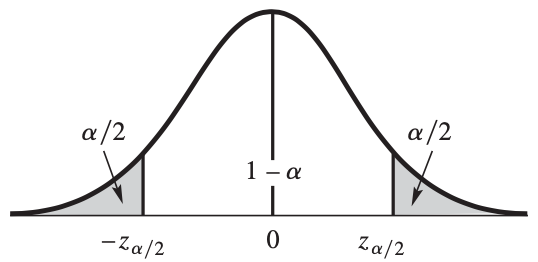
\includegraphics[scale=0.5]{images/z-critical-values.png}
    \end{minipage}
    \begin{minipage}{0.4\textwidth}
        \center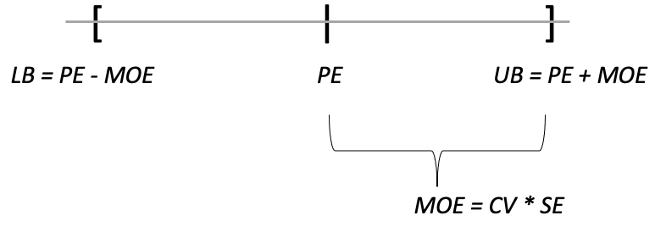
\includegraphics[scale=0.5]{images/ci-general.png}
    \end{minipage}
    \end{figure}

    \item Summary of CIs
    \begin{itemize}
        \item Point Estimate (PE) is the best guess; at the center of the interval.
        \item Margin of Error (MOE) = Critical Value (CV) $\times$ Standard Error (SE).
        \item[] SE (standard deviation of the statistic) measures sampling error.
        \item[] \% Confident is determined by confidence level set and incorporated via the critical value (CV).
    \end{itemize}
    \item All else equal, here is how the researcher can affect the precision of intervals:
    \begin{itemize}
        \item Larger sample size $n$ $\rightarrow$ smaller interval (smaller SE)
        \item More confident $\rightarrow$ larger interval (larger CV)
        \begin{figure}[H]
            \center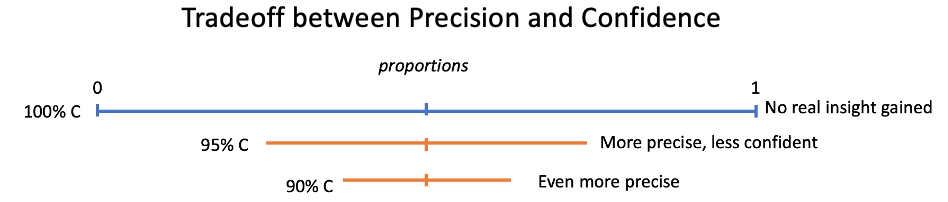
\includegraphics[scale=0.5]{images/confidence-vs-precision.png}
        \end{figure}
    \end{itemize}
    \item Interpretation general structure:
    \item[] I am \ul{\% confident} that the true/population \ul{parameter + context} is between \\ \ul{lower bound} and \ul{upper bound}.
\end{itemize}\bigskip

Types of intervals
\begin{itemize}
    \item Variables that affect the form of intervals:
    \begin{itemize}
        \item Independent or dependent samples
        \item Sample sizes $n_1$ and $n_2$ (large or small)
        \item Population distributions $X_1$ and $X_2$ (normal or not normal)
        \item Population variances $\sigma^2_1$ and $\sigma^2_2$ (known or unknown and ratio of variances)
    \end{itemize}
    \item Large sample confidence intervals
    \item[] If $n$ is large $\Longrightarrow$ $\hat{\theta} \followsp{approx}{Normal}(\theta, \sigma_{\hat{\theta}}) \Longrightarrow 100 (1 - \alpha)\% \text{ CI } = \hat{\theta} \pm z_{\alpha / 2} \, \sigma_{\hat{\theta}}$
    \item[] Conditions: for means $n_i \ge 30$; for proportions $n_i p_i \ge 5$ and $n_i (1 - p_i) \ge 5$ \bigskip\\
    \begin{tabular}{llll}
    $\theta$ & $\hat{\theta}$ & $\sigma_{\hat{\theta}}$ & \\
    \hline\\
    $\mu$ & $\bar{X}$ & $\displaystyle \frac{\sigma}{\sqrt{n}}$ & Estimate $\sigma^2$ with $s^2$ if unknown \\\\
    $\mu_1 - \mu_2$ & $\bar{X}_1 - \bar{X}_2$ & $\displaystyle \sqrt{\frac{\sigma^2_1}{n_1} + \frac{\sigma^2_2}{n_2}}$ & Estimate $\sigma^2_i$ with $s^2_i$ if unknown \\\\
    $p$ & $\hat{p}$ & $\displaystyle \sqrt{\frac{p (1 - p)}{n}}$ & Estimate $p$ with $\hat{p}$ \\\\
    $p_1 - p_2$ & $\hat{p}_1 - \hat{p}_2$ & $\displaystyle \sqrt{\frac{p_1 (1 - p_1)}{n_1} + \frac{p_2 (1 - p_2)}{n_2}}$ & Estimate $p_i$ with $\hat{p}_i$ \\\\
    \end{tabular}
    \item[] If starting from $X_i \follow{Normal}$ and known variances, then intervals are exact; if not then $X_i \approx \text{Normal}$ by CLT and confidence coefficients are approximate.\newpage
    \item Small sample confidence intervals for means ($n_i < 30$)
    \item[] If $n$ is small $\Longrightarrow$ $100 (1 - \alpha)\% \text{ CI } = \hat{\theta} \pm t_{\alpha / 2} \, \sigma_{\hat{\theta}}$ \hspace{100pt} $t$ crit values > $z$ crit values
    \item[] Conditions: for one sample $X \follow{Normal}$ with unknown $\sigma^2$; for two samples $X_1 \ind X_2$ and \\ $X_1, X_2 \follow{Normal}$ with unknown common variance $\sigma^2$
    \begin{figure}[H]
        \center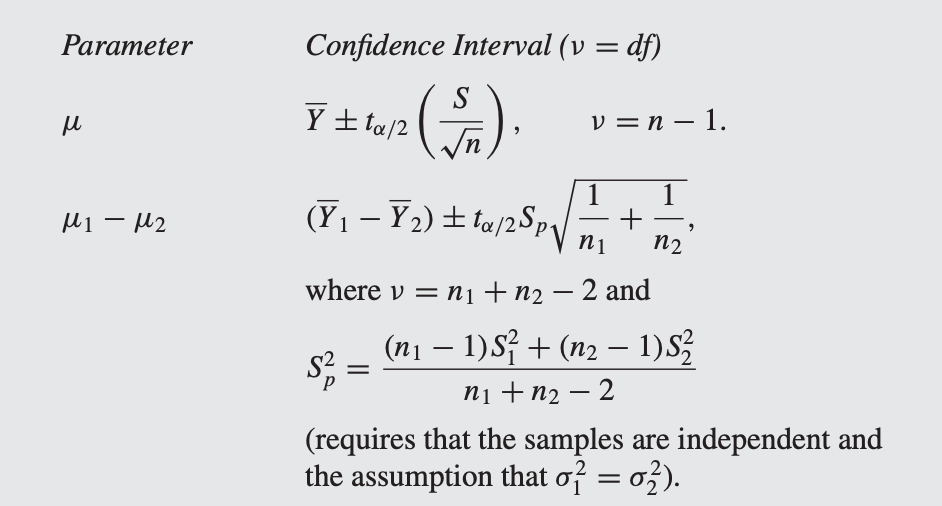
\includegraphics[scale=0.5]{images/small-n-ci.png}
    \end{figure}
    \item[] If not starting from $X_i \follow{Normal}$ then confidence coefficients are approximate and work well as long as not badly skewed with outliers.
    \item Dependent samples CI for $\mu_1 - \mu_2$
    \item[] Simplifies to a one sample CI for the differences $\mu_1 - \mu_ 2 = \mu_D$ shown above if $n$ is small\bigskip
    \item One-sided CI
    \item[] \ul{Lower bound (at least)} \hspace{200pt} \ul{Upper bound (at most)}
    \item[] $P(\hat{\theta} - z_\alpha \, \sigma_{\hat{\theta}}) = 1 - \alpha$  \hspace{150pt} $P(\hat{\theta} + z_\alpha \, \sigma_{\hat{\theta}}) = 1 - \alpha$
    \item[] $\Longrightarrow [\hat{\theta} - z_\alpha \, \sigma_{\hat{\theta}}, \infty)$ \hspace{170pt} $\Longrightarrow (-\infty, \hat{\theta} + z_\alpha \, \sigma_{\hat{\theta}}]$
\end{itemize}\bigskip

Margin of error (MOE) revisited
\begin{itemize}
    \item $MOE = \frac{UB - LB}{2} = \frac{Width}{2} \hspace{20pt} \rightarrow \hspace{20pt} Width = 2 \times MOE$
    \item The \textbf{error in estimation} $\boldsymbol{\epsilon}$ is the distance between an estimator and its target parameter:
    \item[] $[\hat{\theta} - \epsilon, \hat{\theta} + \epsilon] \Longrightarrow \lvert \hat{\theta} - \theta \rvert = \epsilon$
\end{itemize}\bigskip

Finding minimum sample size
\begin{itemize}
    \item We want the $100 (1 - \alpha)\%$ confidence interval for $\theta$, $\hat{\theta} \pm z_{\alpha / 2} \sigma_{\hat{\theta}}$, to be no longer than that given by $\hat{\theta} \pm \epsilon$, then for
    \begin{itemize}
        \item One mean $\mu$ with $V(X) = \sigma^2$ known and $X \follow {Normal}$ or assume going to have ``large'' $n$:
        \item[] $\displaystyle n \ge \frac{z_{\alpha / 2}^2 \sigma^2}{\epsilon^2}$
        \item[] If $\sigma^2$ is unknown, use best approximation available.
        \item One proportion $p$: $\displaystyle n \ge \frac{z_{\alpha / 2}^2 \, p^* (1 - p^*)}{\epsilon^2}$
        \item[] If there is prior knowledge, use $p^* = \hat{p}$, else set $p^* = 0.5$
    \end{itemize}
\end{itemize}

\newpage

{\large \bu{Lecture 7 -- Hypothesis Tests}} (8.1 - 8.3)\bigskip

Hypothesis test
\begin{itemize}
    \item Definition: A hypothesis test is a rule that specifies
    \item[] For which sample value the decision is made to reject $\ho$ in favor of $\ha$.
    \item[] For which sample value the decision is made to ``not reject'' $\ha$ in favor of $\ha$.
    \item Elements of a hypothesis test
    \begin{enumerate}
        \item Null hypothesis $\ho$ and Alternative hypothesis $\ha$
        \item[] Definitions:
        \begin{itemize}
            \item Hypotheses are statements about population parameters
            \item The Null hypothesis $\ho$ is an assumption about $\theta$ that is assumed to be true
            \item The Alternative hypothesis $\ha$ is the complement of $\ho$
        \end{itemize}
        \item Test statistic (TS) and Rejection Region $RR$
        \item[] TS: Function of the sample $W(\vecn{X}{n})$, think of this as the point estimator $\hat{\theta}$
        \item[] RR: Subset of the sample space (range of sample) for which $\ho$ will be rejected
        \item Conclusion / interpretation
        \item[] General structure: Because our test statistic \ul{(COMPARISON of TS and RR)} \ul{(IS / IS NOT)} in the rejection region we \ul{(REJECT or FAIL TO REJECT)} the null hypothesis. \\ At the \ul{(ALPHA)} significance level, there \ul{(IS or IS NOT)} sufficient evidence to conclude \ul{(THE ALTERNATIVE HYPOTHESIS)}.
    \end{enumerate}
\end{itemize}\bigskip

Large sample tests
\begin{itemize}
    \item If $n$ is large, then $\hat{\theta} \follow{Normal}(\theta, \sigma_{\hat{\theta}})$ (or approximately normal) $\Longrightarrow$ $Z = \frac{\hat{\theta} - \theta}{\sigma_{\hat{\theta}}} \follow{Normal}(0,1)$
    \item Using the same parameters $\theta$, point estimates $\hat{\theta}$, and standard errors $\sigma_{\hat{\theta}}$ as shown in confidence intervals, all of the large sample $\alpha$-level tests can be summarized with
    \begin{figure}[H]
    \begin{minipage}{0.45\textwidth}
        \center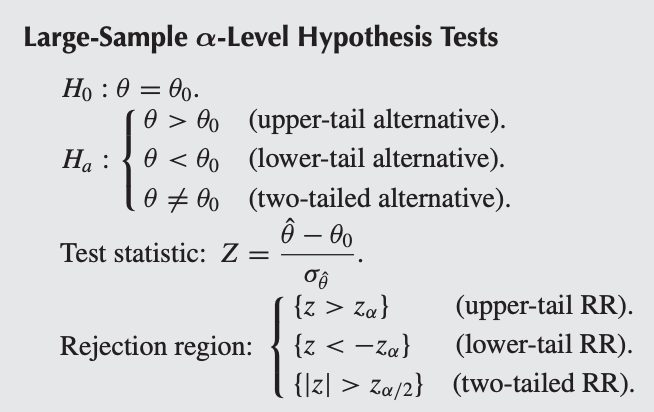
\includegraphics[scale=0.5]{images/large-sample-tests-summary.png}
    \end{minipage}
    \begin{minipage}{0.4\textwidth}
        \center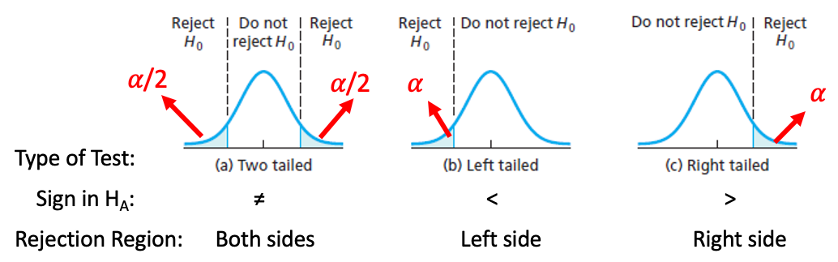
\includegraphics[scale=0.4]{images/rr.png}
    \end{minipage}
    \end{figure}
    \item For proportions
    \begin{itemize}
        \item One sample: In the standard error, use $p_0$ $\Longrightarrow \displaystyle \sigma_{\hat{p}} = \sqrt{\frac{p_0 (1 - p_0)}{n}}$.
        \item Two sample: In the standard error, use $p_1 = p_2 = p$ and estimate with \\$\displaystyle \hat{p} = \frac{x_1 + x_2}{n_1 + n_2} \Longrightarrow \sigma_{\hat{p}_1 - \hat{p}_2} = \sqrt{\hat{p} (1 - \hat{p}) [1 / n_1 + 1 / n_2]}$.
    \end{itemize}\newpage
    \item In any particular test, only one of the listed alternatives $\ha$ is appropriate, which will be based on the research question. Then use the corresponding rejection region.
\end{itemize}\bigskip

Small sample tests for means
\begin{itemize}
    \item If $n$ is small, then need to switch to $t$-tests. For these we start with $X \follow{Normal}$
    \item Summary of the small-sample $\alpha$-level tests for $\mu$
    \begin{figure}[H]
        \center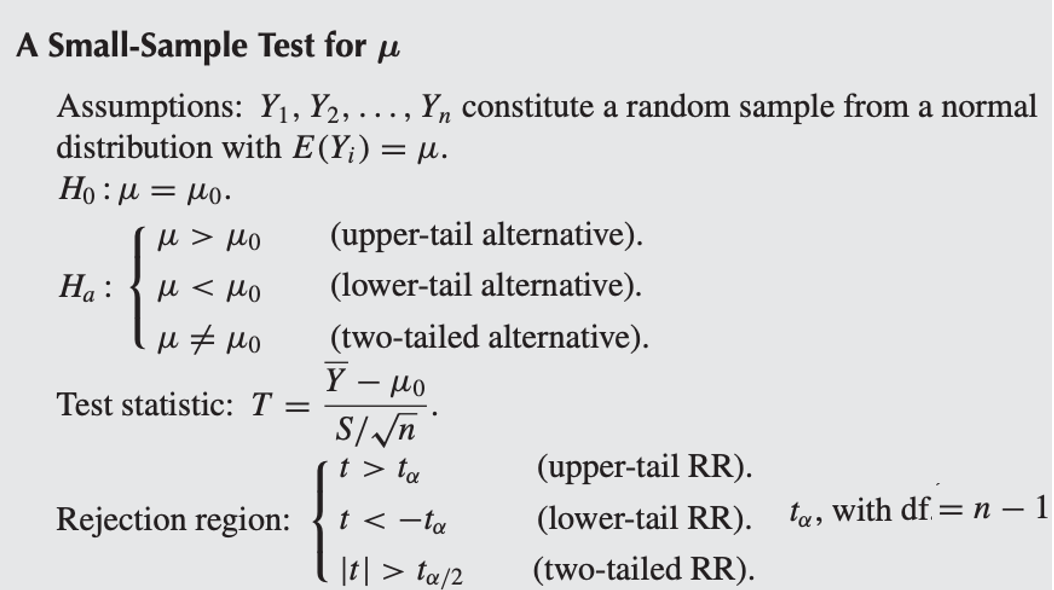
\includegraphics[scale=0.5]{images/small-sample-tests-summary-one-mean.png}
    \end{figure}
    \item If we are testing two independent means $\mu_1 - \mu_2$ and assume both Normal distributions with common unknown variance $\sigma^2$, then we use the pooled variance $S^2_p$ as the estimator for $\sigma^2$ in the standard error $\sigma_{\bar{X}_1 - \bar{X}_2}$. Then
    \begin{figure}[H]
        \center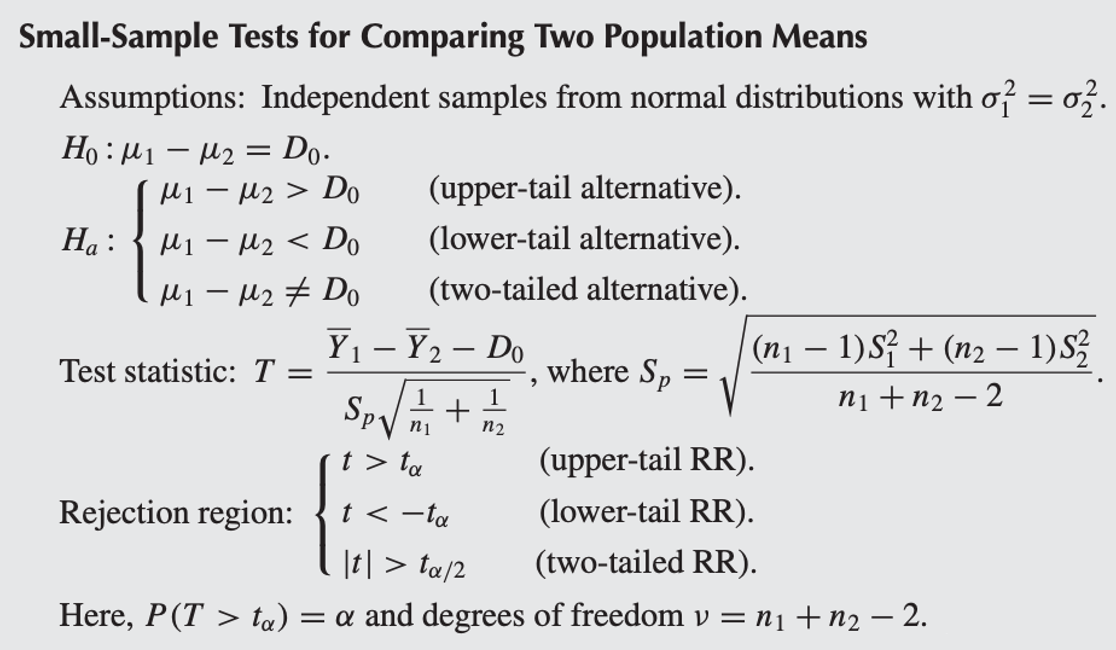
\includegraphics[scale=0.5]{images/small-sample-tests-summary-two-means.png}
    \end{figure}
    \item If we are testing dependent means $\mu_1 - \mu_2$, then have paired $t$-test    \item[] $\mu_1 - \mu_2 = \mu_D \hspace{20pt} \rightarrow \hspace{20pt} \frac{\bar{D} - \mu_D}{S_D / \sqrt{n}} = T \follow{t}_{n-1}$, \hspace{20pt} one sample test on differences
    \item[] If not starting from $X_i \follow{Normal}$ then $t$-tests are approximately $\alpha$-level and work well as long as not badly skewed with outliers.
\end{itemize}\newpage

p-values
\begin{itemize}
    \item Definition: A p-value is the probability that under the null hypothesis the test statistic will be at least as ``extreme'' as the observed value.
    \item Two ways to make conclusion for hypothesis tests:
    \item[] Traditional method: $TS \overset{?}\in RR$
    \item[] p-value method: Reject $\ho$ if p-value $\le \alpha$ \hspace{10pt} and \hspace{10pt} Fail to reject $\ho$ if p-value $> \alpha$
\end{itemize}\bigskip

Relationship between confidence intervals and hypothesis tests
\begin{itemize}
    \item Confidence interval = Acceptance region = Complement of RR
    \item Decisions based on CI: For $\ho: \theta = \theta_0$ and
    \item[] Two-tailed $\ha: \theta \ne \theta_0$: ``Accept'' $\ho$ if $\theta_0$ falls within the $100 (1 - \alpha)$\% CI and reject if outside.
    \item[] Right-tailed $\ha: \theta > \theta_0$: Reject if outside lower bound CI
    \item[] Right-tailed $\ha: \theta < \theta_0$: Reject if outside upper bound CI
\end{itemize}\bigskip

Type I and Type II errors
\begin{itemize}
    \item Type I: Incorrectly rejecting $\ho$
    \item[] $\alpha = P(\text{Type I error}) = P(\text{Reject when $\ho$ is true}) = P(TS \in RR \mid \ho)$
    \item Type II: Incorrectly failing to reject $\ho$
    \item[] $\beta = P(\text{Type II error}) = P(\text{Fail to reject when $\ho$ is false}) = P(TS \notin RR \mid \ha)$
    \begin{figure}[H]
        \center Example for one mean
        \center\includegraphics[scale=0.5]{{"images/type1-type2"}.png}
    \end{figure}
    \item Power: Correctly rejecting $\ho$
    \item[] $\text{Power} = 1 - \beta = P(\text{Reject $\ho$ when $\ho$ is false}) = P(TS \in RR \mid \ha)$
\end{itemize}\newpage

{\large \bu{Lecture 8 -- Regression}} (new textbook)\bigskip

Initial model statement: $Y_i = \beta_0 + \beta_1 X_i + \epsilon_i$
\begin{itemize}
    \item Pieces
    \begin{itemize}
        \item $Y_i$: Dependent (or response) variable value.
        \item $X_i$: Independent (or predictor) variable value. 
        \item $\epsilon_i$: Random error term, \textbf{assumed} to have mean zero and variance $\sigma^2$. \\$\mathrm{Cov}(\epsilon_i, \epsilon_j) = \mathrm{Corr}(\epsilon_i, \epsilon_j) = 0$ for all $i,j : i \ne j$.
        \item $\beta_0$: $Y$-intercept of the regression line and gives $Y$'s mean when $X = 0$
        \item $\beta_1$: Slope of the regression line and indicates the change in $Y$'s \textbf{mean} when $X$ increases by one unit.
        \item $\sigma^2$: Error variance.
    \end{itemize}
    \item Implications
    \begin{itemize}
        \item Mean of $Y_i$ for given $X_i$ $\rightarrow$ $E(Y_i) = \beta_0 + \beta_1 X_i$
        \item Variance of $Y_i$ for given $X_i$ $\rightarrow$ $V(Y_i) = \sigma^2$
    \end{itemize}
\end{itemize}\bigskip

Estimation of the regression function
\begin{itemize}
    \item Method of least squares
    \begin{itemize}
        \item Goal: Minimize function of errors $\displaystyle Q = \sum_{i = 1}^n (Y_i - \beta_0 - \beta_1 X_i)^2$
        \item Results:
        \begin{align*}
            \text{Intercept} \hspace{10pt} \hat{\beta}_0 \hspace{10pt} &= \hspace{10pt} \frac{1}{n}\sum Y_i + \hat{\beta}_1 \frac{1}{n} \sum X_i \hspace{10pt} = \hspace{10pt} \bar{Y}- \hat{\beta}_1 \bar{X} \\
            \text{Slope} \hspace{10pt} \hat{\beta_1} \hspace{10pt} &= \hspace{10pt} \frac{\sum X_i Y_i -\frac{1}{n} \sum X_i Y_i}{\sum X_i^2 - \frac{1}{n}(\sum X_i)^2} \hspace{10pt} = \hspace{10pt} \frac{\sum(X_i - \bar{X})(Y_i - \bar{Y})}{\sum(X_i - \bar{X})^2} \hspace{10pt} = \hspace{10pt} \frac{S_{XY}}{S_{XX}}
        \end{align*}
   \end{itemize}
\end{itemize}\bigskip

Residuals and estimating error variance
\begin{itemize}
    \item Residuals are the known, observable estimate of the unobservable model error: $\hat{\epsilon}_i = e_i = Y_i - \hat{Y}_i$
    \item[] These are very useful for studying whether the given regression model is appropriate for the data.
    \item Estimating error variance:
    \item[] $\displaystyle \text{Error (residual) mean square} \hspace{10pt} S^2 = MSE = \frac{SSE}{n - 2} = \frac{\sum_{i = 1}^n (Y_i - \hat{Y_i})^2}{n - 2} = \frac{\sum_{i = 1}^n e_i^2}{n - 2}$
    \begin{itemize}
        \item Unbiased: $E(MSE) = \sigma^2$
    \end{itemize} 
    \item[] and $S = \sqrt{MSE}$
\end{itemize}\newpage

Normal error regression model\bigskip
\begin{itemize}
    \item $Y_i = \beta_0 + \beta_1 X_i + \epsilon_i, \hspace{20pt} \text{where} \hspace{10pt} \epsilon_i \overset{iid}\sim \text{Normal}\,(0,\sigma^2)$
    \item MLEs of regression parameters and error variance\bigskip\\
    \begin{tabular}{l l}
        Parameter  & MLE\\
        \hline
        $\beta_0$ & $\hat{\beta}_0 \hspace{10pt}$ Same as LSE\\
        $\beta_1$  & $\hat{\beta}_1 \hspace{10pt}$ Same as LSE\\
        $\sigma^2$ & $\displaystyle \hat{\sigma}^2 = \frac{\sum (Y_i - \hat{Y_i})^2}{n}$\\
    \end{tabular}
\end{itemize}\bigskip

Inference (tests on $\beta_1$)
\begin{itemize}
    \item Sampling distribution of standardized $\hat{\beta}_1$: $(\hat{\beta}_1 - \beta_1) / S_{\hat{\beta}_1}$
    \item[] $\displaystyle \frac{\hat{\beta}_1 - E(\hat{\beta}_1)}{SE(\hat{\beta}_1)} = \frac{\hat{\beta}_1 - \beta_1}{S_{\hat{\beta}_1}} = \frac{\hat{\beta}_1 - \beta_1}{\sqrt{MSE / S_{XX}}} \sim \text{t}\,_{n - 2}$
    \item Two-tailed test (most common)
    \begin{itemize}
        \item Hypotheses
        \begin{align*}
          H_0 &: \beta_1 = 0 \\
          H_A &: \beta_1 \ne 0
        \end{align*}
        \item Test statistic
        \[
        TS = t^* = \frac{\hat{\beta}_1 - 0}{S_{\hat{\beta}_1}} = \frac{\hat{\beta}_1}{\sqrt{MSE / S_{XX}}}
        \]
        \item Rejection region and p-value
        \begin{align*}
          RR &= \{\lvert t \rvert > t_{\alpha/2, n - 2}\} \\
          p\text{-value} &= 2 \cdot P(t_{n-2} \ge \lvert t \rvert)
        \end{align*}
        \item Decision
        \begin{itemize}
            \item Reject $H_0$ and conclude $H_A$ if $\hspace{10pt}$ $TS \in RR \hspace{10pt} \Longleftrightarrow \hspace{10pt} p\text{-value} \le \alpha$
            \item Fail to reject $H_0$ if $\hspace{10pt}$ $TS \notin RR \hspace{10pt} \Longleftrightarrow \hspace{10pt} p\text{-value} > \alpha$
            \item Can also look at the $100(1 - \alpha)\%$ CI for $\beta_1$ to see if contains 0.
        \end{itemize}
        \item Conclusion / Interpretation
        \item[] At the $\alpha$ significance level, we < have / do not have > sufficient evidence of a significant linear relationship between < $Y$ context > and < $X$ context >. < if yes... > This is a < positive / negative > linear relationship, indicating that as < $X$ context > increases, < $Y$ context > < increases / decreases >, on average.
    \end{itemize}
\end{itemize}\bigskip

Descriptive measures of linear association between $X$ and $Y$
\begin{itemize}
    \item Coefficient of determination $R^2$
    \item[] $\displaystyle R^2 = \frac{SSR}{SSTO} = 1-\frac{SSE}{SSTO}, \hspace{20pt} \text{range:} \hspace{10pt} 0 \le R^2 \le 1$
\end{itemize}\
\newpage

Diagnostics
\begin{itemize}
    \item Diagnostics = assumption checking
    \item[] Residuals should model the properties of $\epsilon_i \followsp{iid}{Normal}\,(0, \sigma^2$)
    \begin{itemize}
        \item LINE $\rightarrow$ Linearity, Independence, Normality, Equal variance
    \end{itemize}
    \item Ideal residual plots if all assumptions on the error terms are met: 
    \begin{figure}[H]
        \center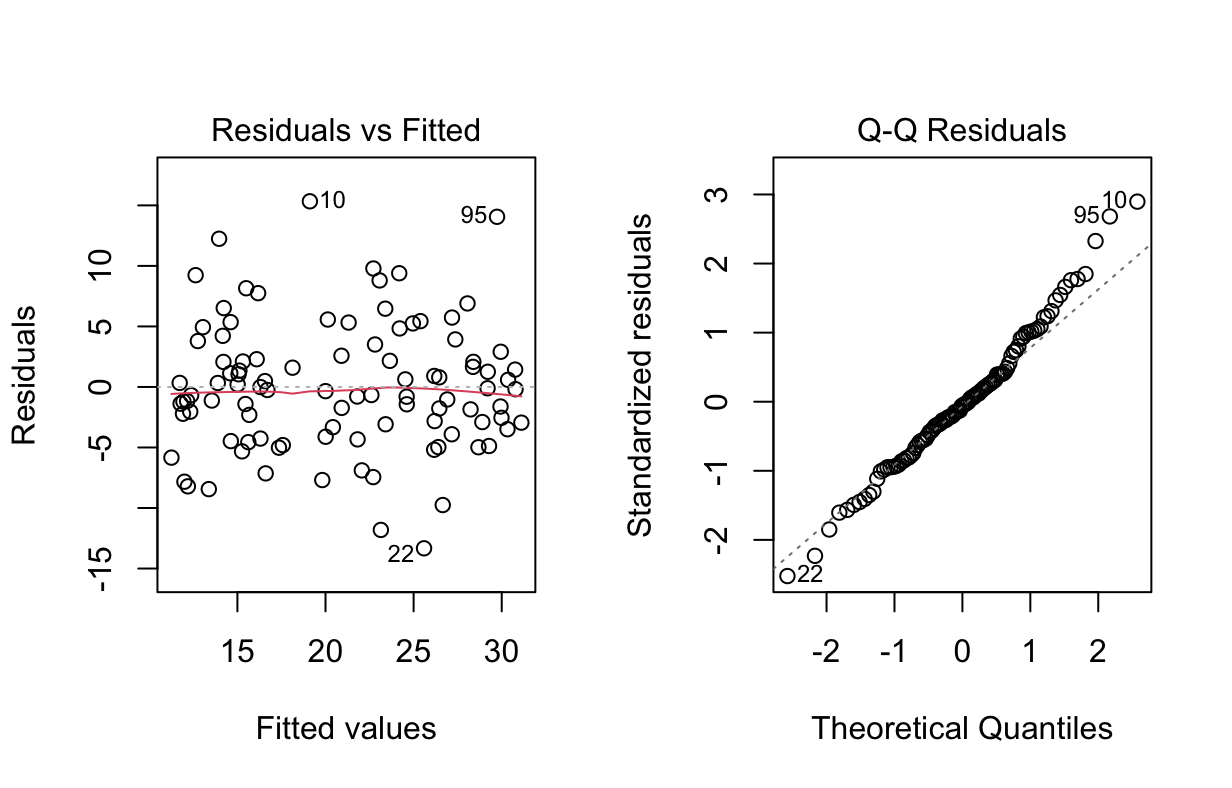
\includegraphics[scale=0.25]{images/ideal-diagnostics.png}
    \end{figure}
\end{itemize}\bigskip

% same distribution table as last test -> so skipping here

\end{document}




